\documentclass[11pt]{article}
\pagestyle{empty}

\oddsidemargin -0.25in
\textwidth 7.0in         
\topmargin 0.0in
\headheight 0.0in
\headsep 0.0in
\topskip 0.0in
\footskip 0.4in
\textheight 8.8in         

\usepackage{mathtools}
\usepackage{graphicx}  %for including .jpeg files
\usepackage[algoruled,vlined,linesnumbered,commentsnumbered]{algorithm2e}
\usepackage{xcolor}
\usepackage{tikz}
\usepackage{pgfplots}

\begin{document}
\noindent
{\large\bf Encrypted Joins with FHIPE} 

\noindent
Experiment Results from Hash-Based Implementation (Fall 2020)

\hfill\hrule
\noindent
$\\\\$
In the following plots, $s$ represents selectivity, such that \[s = \frac{|\sigma_{(x \ \texttt{IN} \ \mathbf{x})}|}{|PK|},\]
for some set $\mathbf{x}$.
$\\\\\\$
\textbf{Total Running Time vs. Scale Factor, by Selectivity}
\begin{center}
  \pgfplotsset{scaled x ticks=false}
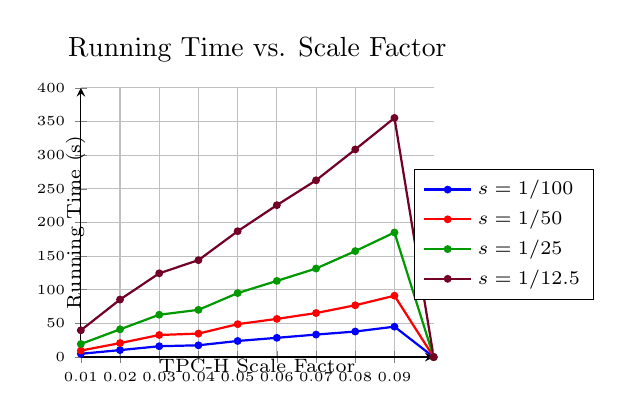
\begin{tikzpicture}
\begin{axis}[
    title=Running Time vs. Scale Factor,
    width=0.5\linewidth,
    height=5cm,
    axis lines=left,
    grid=both,
    legend style={font=\scriptsize},
    legend cell align=left,
    legend style={at={(1.2,0.7)}, anchor=north},
    label style={font=\scriptsize},
    ticklabel style={font=\tiny},
    xlabel style={at={(0.5, 0.03)}},
    ylabel style={at={(0.04, 0.5)}},
    ymin=0,
    ymax=400, %%%%%%%%%%%%%%%%%%%%%%%%%%%%%%%%%%%%%%%%%%%%%%%%%%%% INCREASE THIS TO INCREASE Y-AXIS MAX
    ytick={0,50,...,400},
    xmin=0.01,
    xmax=0.1,
    xtick={0.01, 0.02, 0.03, 0.04, 0.05, 0.06, 0.07, 0.08, 0.09, 0,1},
    xticklabels={0.01, 0.02, 0.03, 0.04, 0.05, 0.06, 0.07, 0.08, 0.09, 0.1},
    xlabel=TPC-H Scale Factor,
    ylabel=Running Time (s),
    legend entries={{$s = 1/100$}, {$s=1/50$}, {$s=1/25$}, {$s=1/12.5$}},
]
\addplot[color=blue, mark=*, thick, mark options={scale=0.5}] coordinates {
  (0.01, 4.85) (0.02, 10.30) (0.03, 16.08) (0.04, 17.46) (0.05, 23.89) (0.06, 28.57) (0.07, 33.40) (0.08, 37.92) (0.09, 45.15) (0.1, 0)};
\addplot[color=red, mark=*, thick, mark options={scale=0.5}] coordinates {
  (0.01, 9.64) (0.02, 20.73) (0.03, 32.76) (0.04, 34.88) (0.05, 48.86) (0.06, 56.68) (0.07, 65.40) (0.08, 76.93) (0.09, 91.16) (0.1, 0)};
\addplot[color=black!40!green, mark=*, thick, mark options={scale=0.5}] coordinates {
  (0.01, 19.37) (0.02, 41.20) (0.03, 62.88) (0.04, 70.12) (0.05, 95.02) (0.06, 113.16) (0.07, 131.54) (0.08, 157.45) (0.09, 185.11) (0.1, 0)};
\addplot[color=black!40!purple, mark=*, thick, mark options={scale=0.5}] coordinates {
  (0.01, 39.70) (0.02, 85.44) (0.03, 124.47) (0.04, 144.00) (0.05, 186.98) (0.06, 225.69) (0.07, 262.65) (0.08, 308.48) (0.09, 355.35) (0.1, 0)};
\end{axis}
\end{tikzpicture}
\end{center}

$\\\\$
\textbf{Total Running Time vs. In Clause Max Size, by Selectivity}
\begin{center}
  \pgfplotsset{scaled x ticks=false}
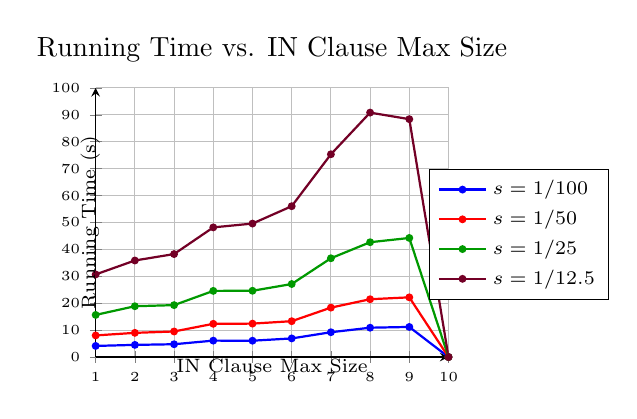
\begin{tikzpicture}
\begin{axis}[
  title=Running Time vs. IN Clause Max Size,
    width=0.5\linewidth,
    height=5cm,
    axis lines=left,
    grid=both,
    legend style={font=\scriptsize},
    legend cell align=left,
    legend style={at={(1.2,0.7)}, anchor=north},
    label style={font=\scriptsize},
    ticklabel style={font=\tiny},
    xlabel style={at={(0.5, 0.03)}},
    ylabel style={at={(0.04, 0.5)}},
    ymin=0,
    ymax=100, %%%%%%%%%%%%%%%%%%%%%%%%%%%%%%%%%%%%%%%%%%%%%%%%%%%% INCREASE THIS TO INCREASE Y-AXIS MAX
    ytick={0,10,...,100},
    xmin=1,
    xmax=10,
    xtick={1, 2, 3, 4, 5, 6, 7, 8, 9, 10},
    xticklabels={1, 2, 3, 4, 5, 6, 7, 8, 9, 10},
    xlabel=IN Clause Max Size,
    ylabel=Running Time (s),
    legend entries={{$s = 1/100$}, {$s=1/50$}, {$s=1/25$}, {$s=1/12.5$}},
]
\addplot[color=blue, mark=*, thick, mark options={scale=0.5}] coordinates {
  (1, 4.13) (2, 4.52) (3, 4.76) (4, 6.10) (5, 6.07) (6, 6.92) (7, 9.22) (8, 10.90) (9, 11.18) (10, 0)};
\addplot[color=red, mark=*, thick, mark options={scale=0.5}] coordinates {
  (1, 8.03) (2, 8.99) (3, 9.50) (4, 12.35) (5, 12.42) (6, 13.32) (7, 18.36) (8, 21.48) (9, 22.18) (10, 0)};
\addplot[color=black!40!green, mark=*, thick, mark options={scale=0.5}] coordinates {
  (1, 15.65) (2, 18.88) (3, 19.29) (4, 24.58) (5, 24.62) (6, 27.13) (7, 36.70) (8, 42.66) (9, 44.24) (10, 0)};
\addplot[color=black!40!purple, mark=*, thick, mark options={scale=0.5}] coordinates {
  (1, 30.69) (2, 35.87) (3, 38.26) (4, 48.17) (5, 49.59) (6, 56.04) (7, 75.33) (8, 90.81) (9, 88.38) (10, 0)};
\end{axis}
\end{tikzpicture}
\end{center}

\end{document}
